\documentclass[a4paper,11pt]{article}
\usepackage{fancyhdr}
\usepackage[utf8x]{inputenc}
\usepackage[croatian]{babel}
\usepackage{fancyhdr}
\usepackage{amsmath}
\usepackage{amssymb}
\usepackage{mathrsfs}
\usepackage[croatian]{babel}
\usepackage{graphicx}
\newcommand{\arctg}[1]{\text{arctg}(#1) }
\newcommand{\tg}[1]{\text{tg}(#1)}
\usepackage{amsmath,amssymb}
\usepackage{amsthm}
\usepackage{thmtools}
\usepackage{tikz,lipsum,lmodern}
\usepackage[most]{tcolorbox}
\usepackage[T1]{fontenc}
\usepackage{color}
\usepackage{gensymb}
\renewcommand\familydefault{\sfdefault}
\usepackage{tgheros}
\renewcommand\familydefault{\sfdefault}
\usepackage{tgheros}
\usepackage[dvipsnames]{xcolor}

\usepackage{tcolorbox}
\definecolor{mycolor}{rgb}{1.0, 0.49, 0.0}
\newtcbox{\mybox}{on line,
  colframe=mycolor,colback=mycolor!30!white,
  boxrule=0.7pt,arc=4pt,boxsep=0pt,left=6pt,right=6pt,top=6pt,bottom=6pt}
\colorlet{Mycolor1}{yellow!60!orange!40!}
\definecolor{Mycolor2}{HTML}{00F9DE}



\usepackage{amsmath,amssymb,amsthm,textcomp}
\usepackage{enumerate}
\usepackage{multicol}
\usepackage{tikz}

\usepackage{geometry}
\geometry{left=25mm,right=25mm,%
bindingoffset=0mm, top=20mm,bottom=20mm}




\usepackage{hyperref}
\hypersetup{
    colorlinks=true,
    linkcolor=blue,
    urlcolor=red,
    linktoc=all
}

\definecolor{background}{RGB}{225,225,220}
\pagecolor{background}
\fboxsep=2mm
\declaretheoremstyle[
spaceabove=6pt, spacebelow=6pt,
headfont=\normalfont\bfseries,
notefont=\mdseries, notebraces={(}{)},
bodyfont=\normalfont,
postheadspace=1em,
numberwithin=section
]{exstyle}
\declaretheoremstyle[
spaceabove=6pt, spacebelow=6pt,
headfont=\normalfont\bfseries,
notefont=\mdseries, notebraces={(}{)},
bodyfont=\normalfont,
postheadspace=2em,
headpunct={},
qed=$\blacktriangleleft$,
numbered=no
]{solstyle}
\declaretheorem[style=exstyle]{zadatak}
\declaretheorem[style=solstyle]{rjesenje:}


\pagestyle{fancy}
\fancyhf{}
\fancyhead[LE,RO]{Riješeni zadaci}
\fancyhead[RE,LO]{Matematika II}
\fancyfoot[CE,CO]{\leftmark}
\fancyfoot[LE,RO]{ \thepage}


\renewcommand{\headrulewidth}{2pt}
\renewcommand{\footrulewidth}{2pt}

\begin{document}
\pagecolor{white}
\color{black}







\begin{center}
\tcbox[ colframe=red, colback=white!50!white!30]{\LARGE{PRIMJENA DVOJNOG INTEGRALA}}
\end{center}
\begin{tcolorbox}[enhanced,attach boxed title to top center={yshift=-3mm,yshifttext=-1mm},
  colback=yellow!15!white,colframe=red!755!yellow,colbacktitle=brown!90!white,
  title=Površina,fonttitle=\bfseries,
  boxed title style={size=small,colframe=red!50!black} ]
    Površinu oblasti $D$  računamo se po formuli:

$$ P=\iint\limits_D dx dy.$$ 	   


\end{tcolorbox}
\begin{tcolorbox}[colback=brown!35!white,colframe=white!75!white,title= $$\bullet \bullet \bullet$$]
         \begin{zadatak}
Izvesti formulu za površinu elipse:
$$\frac{x^{2}}{a^{2}} + \frac{y^{2}}{b^{2}} = 1.$$
\end{zadatak}
\end{tcolorbox}
\emph{Rješenje: }
\begin{center}
\tcbox[ colframe=red, colback=white!50!white!30]{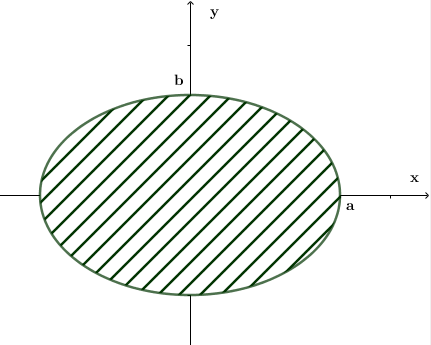
\includegraphics[width=7cm]{c1.png}}
\end{center}
Uvedimo uopštene polarne koordnate:
$$x = a r \cos{\varphi}$$
$$y = br \sin{\varphi}$$
$$J = abr$$
 $$\mathrm dxdy =ab r  \mathrm d r  \mathrm d\varphi$$
 Ako ove koordinate uvrstimo u jednačinu elipse, naći ćemo granice za r, odnosno:
 $$\frac{x^{2}}{a^{2}} + \frac{y^{2}}{b^{2}} = \frac{a^{2} r^{2}\cos^{2}{\varphi}}{a^{2}}  + \frac{ b^{2}r^{2} \sin^{2}{\varphi}}{b^{2}} = r^2 =1 $$
 Prema tome, vrijedi:
 $$0\leq r \leq 1$$
  $$0\leq \varphi \leq 2\pi$$
 

$$P = \iint \limits_{D}   \mathrm dx \mathrm dy = \int\limits_{0}^{2\pi} \mathrm d \varphi  \int\limits_{0}^{1}ab r\mathrm dr$$ 
$$= ab\int\limits_{0}^{2\pi} \mathrm d \varphi   \frac{r^{2}}{2}\Big{|}_{0}^{1} $$
$$ = \frac{ab}{2}\int\limits_{0}^{2\pi} \mathrm d \varphi   = \frac{ab}{2} \cdot 2\pi = ab\pi.\hskip 2 cm \blacktriangleleft  $$


 
 
 \begin{tcolorbox}[colback=brown!35!white,colframe=white!75!white,title= $$\bullet \bullet \bullet$$]
         \begin{zadatak}
Izračunati površinu lika ograničenog sa krivim:\\ $y\leq x$, $y\geq -x$ i $x^{2} + y^{2} \leq 2x.$

\end{zadatak}
\end{tcolorbox}
\emph{Rješenje: }
\begin{center}
\tcbox[ colframe=red, colback=white!50!white!30]{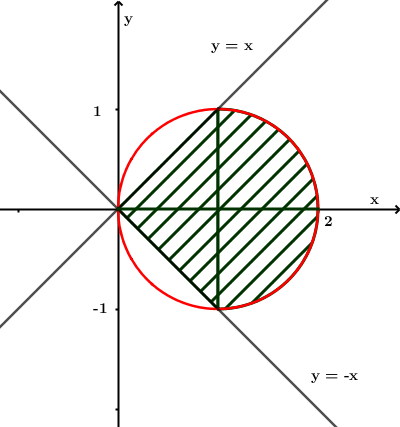
\includegraphics[width=7cm]{c2.png}}
\end{center}
Uvedimo polarne koordinate:
$$x = r \cos{\varphi}$$
$$y = r \sin{\varphi}$$
 $$\mathrm dxdy = r  \mathrm d r  \mathrm d\varphi$$
 Sada trebamo naći granice za $r$  i $\varphi.$ 
 Iz $x^{2} + y^{2} \leq 2x \Rightarrow r\leq 2\cos{\varphi} \Rightarrow 0\leq r \leq 2\cos{\varphi}. $
 Donja granica za ugao $\varphi$ jeste $-\frac{\pi}{4}$, jer je prava $y= -x$ prava pod uglom od $45 \degree$ (ali krećemo se u negativnom smjeru, pa je to $-\frac{\pi}{4}$ )
  Gornja granica za $\varphi$  je  vezana za presječnu tačku prave $y = x$ i kružnice $x^{2} + y^{2} = 2x$. To bi bila tačka $(1,1 ).$ 
$$\Rightarrow \varphi = \arctg{1} = \frac{\pi}{4}.$$
(Iako, znamo da je prava $y=x$ prava pod uglom od $45 \degree$ i mogli smo odmah uočiti da je gornja granica za ugao $\varphi$ $45 \degree = \frac{\pi}{4}.$ )
\\ Ili možemo pronaći granice iz: $$y \leq x \Rightarrow r\sin{\varphi} \leq r\cos{\varphi} \hspace{1 cm} / :r\cos{\varphi}$$
$$tg(\varphi) \leq 1 \Rightarrow \varphi \leq \frac{\pi}{4}$$
Stoga, vrijedi da je tražena površina:
$$P = \iint \limits_{D}   \mathrm dx \mathrm dy = \int\limits_{-\frac{\pi}{4}}^{\frac{\pi}{4}} \mathrm d \varphi  \int\limits_{0}^{2\cos{\varphi}} r\mathrm dr$$ 
$$= \int\limits_{-\frac{\pi}{4}}^{\frac{\pi}{4}} \mathrm d \varphi  \frac{r^{2}}{2} \Big{|}_{0}^{2\cos{\varphi}} = \int\limits_{-\frac{\pi}{4}}^{\frac{\pi}{4}} 2\cos^{2}{\varphi}  \mathrm d \varphi$$
$$   = 2\int\limits_{-\frac{\pi}{4}}^{\frac{\pi}{4}}\frac{ 1 +\cos{2\varphi}}{2}  \mathrm d \varphi  =  \int\limits_{-\frac{\pi}{4}}^{\frac{\pi}{4}} \mathrm d \varphi  + \int\limits_{-\frac{\pi}{4}}^{\frac{\pi}{4}}\cos{2\varphi} \mathrm d \varphi$$
$$= \varphi\Big{|}_{-\frac{\pi}{4}}^{\frac{\pi}{4}} + \frac{1}{2}\sin{2\varphi}\Big{|}_{-\frac{\pi}{4}}^{\frac{\pi}{4}} = \frac{\pi}{2} +\frac{1}{2}\cdot(\sin{\frac{\pi}{2}} + \sin{\frac{\pi}{2}})  = \frac{\pi}{2} + 1. $$
 \textbf{Napomena:} Mogli smo postaviti granice za ugao: 
$$ 0\leq \varphi \leq \frac{\pi}{4} , $$
Tada bismo samo naš intagral pomnožili sa $2$, jer našu oblast integracije možemo podijeliti na   dva potpuno ista dijela  i kada izračunamo površinu gornjeg, znamo da je i površina donjeg dijela ista. Stoga samo udvostručimo tu površinu.

 $\hskip  12 cm  \blacktriangleleft$ \\
  \begin{tcolorbox}[colback=brown!35!white,colframe=white!75!white,title= $$\bullet \bullet \bullet$$]
         \begin{zadatak}
Izračunati površinu lika ograničenog sa krivim:\\ $y\leq x$, $y\geq 0$ , $x^{2} + y^{2} \geq 2x$  i $x^{2} + y^{2} \leq 4x$

\end{zadatak}
\end{tcolorbox}
\emph{Rješenje: }

$$x^{2} + y^{2} = 2x.$$ 
$$x^{2} - 2x + y^{2} = 0.$$ 
$$x^{2} - 2x +1 + y^{2} = 1.$$
$$(x-1)^{2}  + y^{2} = 1.$$
Dakle, ovo je kružnica sa centrom u $(1,0)$, poluprečnika $1,$ i kako je $x^{2} + y^{2} \geq 2x$ u postavci zadatka, to se naša oblast integracije nalazi izvan ove kružnice.
$$x^{2} + y^{2} = 4x.$$ 
$$x^{2} - 4x + y^{2} = 0.$$ 
$$x^{2} - 4x +4 + y^{2} = 4.$$
$$(x-2)^{2}  + y^{2} = 2^{2} = 4.$$
Ovo je kružnica sa centrom u $(2,0)$, poluprečnika $2,$ i kako je $x^{2} + y^{2} \leq 4x$ u postavci zadatka, to se naša oblast integracije nalazi u unutrašnjosti ove kružnice.Zatim, vrijedi  i $y\leq x$, $y\geq 0$ , stoga
nađemo presjek datih uslova, i imamo oblast integracije predstavljenu na slici:

\begin{center}
\tcbox[ colframe=red, colback=white!50!white!30]{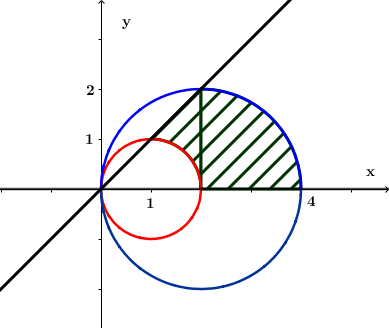
\includegraphics[width=8cm]{c3.png}}
\end{center}

Uvedimo polarne koordinate:
$$x = r \cos{\varphi}$$
$$y = r \sin{\varphi}$$
 $$\mathrm dxdy = r  \mathrm d r  \mathrm d\varphi$$
 Sada trebamo naći granice za $r$  i $\varphi.$ 
Uočimo da granice za $r$ možemo naći iz:  
$$x^{2} + y^{2} \geq 2x \Rightarrow r^{2}\geq 2 r\cos{\varphi}\Rightarrow r\geq 2 \cos{\varphi}$$
$$x^{2} + y^{2} \leq 4x \Rightarrow r^{2}\leq 4 r\cos{\varphi}\Rightarrow r\leq 4 \cos{\varphi}$$

Dakle, vrijedi:
$$ 2 \cos{\varphi} \leq r \leq 4\cos{\varphi} $$
Kad su u pitanju granice za ugao $\varphi$, njih nalazimo iz $$y\leq x \Rightarrow r\sin{\varphi} \leq r\cos{\varphi} \hspace{1 cm} / :r\cos{\varphi} $$
$$tg(\varphi) \leq 1 \Rightarrow \varphi \leq \frac{\pi}{4}$$
Stoga je:
$$ 0 \leq \varphi \leq \frac{\pi}{4} $$
$$P = \iint \limits_{D}   \mathrm dx \mathrm dy = \int\limits_{0}^{\frac{\pi}{4}} \mathrm d \varphi  \int\limits_{2\cos{\varphi}}^{4\cos{\varphi}} r\mathrm dr$$ 
$$= \int\limits_{0}^{\frac{\pi}{4}} \mathrm d \varphi  \frac{r^{2}}{2} \Big{|}_{2\cos{\varphi}}^{4\cos{\varphi}} = \frac{1}{2}\int\limits_{0}^{\frac{\pi}{4}} (16\cos^{2}{\varphi} - 4\cos^{2}{\varphi})  \mathrm d \varphi$$
$$   = 6\int\limits_{0}^{\frac{\pi}{4}}\frac{ 1 +\cos{2\varphi}}{2}  \mathrm d \varphi  =  3\int\limits_{0}^{\frac{\pi}{4}} \mathrm d \varphi  + 3\int\limits_{0}^{\frac{\pi}{4}}\cos{2\varphi} \mathrm d \varphi$$
$$= 3\varphi\Big{|}_{0}^{\frac{\pi}{4}} + 3\cdot \frac{1}{2}\sin{2\varphi}\Big{|}_{0}^{\frac{\pi}{4}} = \frac{3\pi}{4} +\frac{3}{2}\cdot\left(\sin{\frac{\pi}{2}} - \sin{0}\right)  = \frac{3\pi}{4} + \frac{3}{2} . $$
 

 \hskip 12 cm $\blacktriangleleft$ \\
 \begin{tcolorbox}[enhanced,attach boxed title to top center={yshift=-3mm,yshifttext=-1mm},
  colback=yellow!15!white,colframe=red!755!yellow,colbacktitle=brown!90!white,
  title=Zapremina,fonttitle=\bfseries,
  boxed title style={size=small,colframe=red!50!black} ]
    Zapremina tijela $ \Omega$ ograničenog površima $ z=f(x,y)$ i $ z=g(x,y)$ iznad područja $ D$ , pri čemu je $ g(x,y)\leq f(x,y)$ , $ \forall (x,y)\in D$ ,  računa se po formuli:

$$\displaystyle \displaystyle V(\Omega) = \iint\limits_D \left[f(x,y)-g(x,y)\right] dx dy.$$ 	   

\end{tcolorbox}
 \begin{tcolorbox}[colback=brown!35!white,colframe=white!75!white,title= $$\bullet \bullet \bullet$$]
         \begin{zadatak}
Izračunati zapreminu tijela ograničenog sa: \\ $z_1 = x^{2} + y^{2},$ $z_2 = 2(x^{2} + y^{2})$ i $z_3 =4.$
\end{zadatak}
\end{tcolorbox}
\emph{Rješenje: }
Na slici je prikazano tijelo čiju zapreminu želimo izračunati i njegova projekcija na $ xy$ ravan. 
\begin{center}
\tcbox[ colframe=red, colback=white!50!white!30]{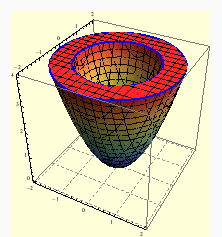
\includegraphics[width=6cm]{d2.png},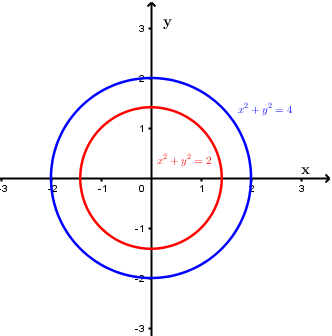
\includegraphics[width=6cm]{d5.png}}
\end{center}


Uvedimo polarne koordinate:
$$x = r \cos{\varphi}$$
$$y = r \sin{\varphi}$$
 $$\mathrm dxdy = r  \mathrm d r  \mathrm d\varphi$$
\begin{center}
\tcbox[ colframe=red, colback=white!50!white!30]{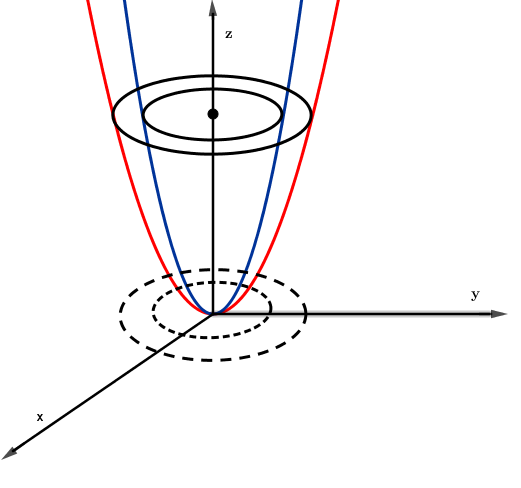
\includegraphics[width=6cm]{c4.png}}
\end{center}
 Jednačina kružnice $ x^2+y^2=4$ u novim koordinatama glasi $ r=2$ , a jednačina kružnice $ x^2+y^2=2$ glasi $ r=\sqrt 2$ .
Zapremina  tijela ograničenog širim paraboloidom $ z=x^2+y^2$ i ravni $ z=4$ jednaka je:

$$ V_{1} 	 =\iint\limits_{ D }\left( z_{ravni}- z_{paraboloida}\right) dx dy=\iint\limits_{D}\left( 4-x^{2}-y^{2}\right) dx dy$$ 	   
  	$$ =\int\limits_{0}^{2\pi } d\varphi \int\limits_{0}^{2}( 4-r^{2})r dr =\int\limits_{0}^{2\pi }\left(4\frac{r^{2}  }{2} - \frac{r^{4}  }{4} \right) \underset{0}{\overset{2 }{ \bigg\vert}}d\varphi =4\varphi \underset{0}{\overset{2\pi }{ \bigg\vert}}=8\pi,$$ 	   
  	 	   

a zapremina tijela ograničenog užim paraboloidom $ z=2(x^2+y^2)$ i ravni $ z=4$ jednaka je:

$$ V_{2} =\iint\limits_{D}\left[ 4-2\left( x^{2}+y^{2}\right) \right] dx dy =  =\int\limits_{0}^{2\pi } d\varphi \int\limits_{0}^{\sqrt{2}}(4 - 2r^{2})r dr$$ 	   
  
  
  	$$=\int\limits_{0}^{2\pi }\left(4\frac{r^{2}  }{2} - 2\frac{r^{4}  }{4} \right) \underset{0}{\overset{\sqrt{2} }{ \bigg\vert}}d\varphi = \int\limits_{0}^{2\pi } 2 d\varphi = 2\varphi \underset{0}{\overset{2\pi }{ \bigg\vert}} = 4\pi.  $$ 	   

Tražena zapremina je: $$ V=V_{1}-V_{2}=8\pi -4\pi =4\pi.$$



\hskip 12 cm $\blacktriangleleft$ \\
 \begin{tcolorbox}[colback=brown!35!white,colframe=white!75!white,title= $$\bullet \bullet \bullet$$]
         \begin{zadatak}
Izračunati zapreminu tijela ograničenog sa: \\ $z_1 = x^{2} + y^{2} $  i $z_2 =4.$
\end{zadatak}
\end{tcolorbox}
\emph{Rješenje: }
\begin{center}
\tcbox[ colframe=red, colback=white!50!white!30]{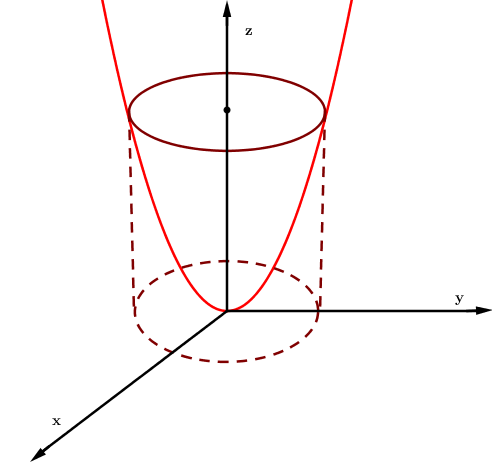
\includegraphics[width=6cm]{c5.png},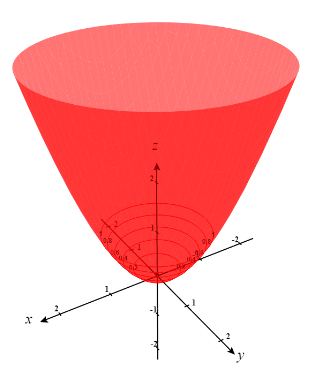
\includegraphics[width=5cm]{d6.png}}
\end{center}
Uvedimo polarne koordinate:
$$x = r \cos{\varphi}$$
$$y = r \sin{\varphi}$$
 $$\mathrm dxdy = r  \mathrm d r  \mathrm d\varphi$$
 Kako bismo odredili granice za $r$ i $\varphi$, moramo naći presjek ravni $z_2 = 4$ i paraboloida. Jednačina presjeka je:
 $$ x^{2} + y^{2} = 4 \Rightarrow r^{2} = 4 \Rightarrow r =2.$$
 $$0 \leq r \leq 2.$$
 Vidimo da nemamo ograničenja za ugao $\varphi$, pa je:
 $$0 \leq \varphi \leq 2\pi$$
 Stoga je tražena zapremina:
$$ V 	 =\iint\limits_{ D }\left( z_{ravni}- z_{paraboloida}\right) dx dy=\iint\limits_{D}\left( 4-x^{2}-y^{2}\right) dx dy$$ 	   
  	$$ =\int\limits_{0}^{2\pi } d\varphi \int\limits_{0}^{2}( 4-r^{2})r dr =\int\limits_{0}^{2\pi }\left(4\frac{r^{2}  }{2} - \frac{r^{4}  }{4} \right) \underset{0}{\overset{2 }{ \bigg\vert}}d\varphi =4\varphi \underset{0}{\overset{2\pi }{ \bigg\vert}}=8\pi.$$ 	

\hskip 12 cm $\blacktriangleleft$ \\
 \begin{tcolorbox}[colback=brown!35!white,colframe=white!75!white,title= $$\bullet \bullet \bullet$$]
         \begin{zadatak}
Izvesti izraz za zapreminu sfere(lopte).
\end{zadatak}
\end{tcolorbox}
\emph{Rješenje: }
Jednačina centralne sfere je: 
$$x^2 + y^2 + z^2 = r^2 \Rightarrow z = \pm \sqrt{r^{2} - x^2 - y^2 } .$$

\begin{center}
\tcbox[ colframe=red, colback=white!50!white!30]{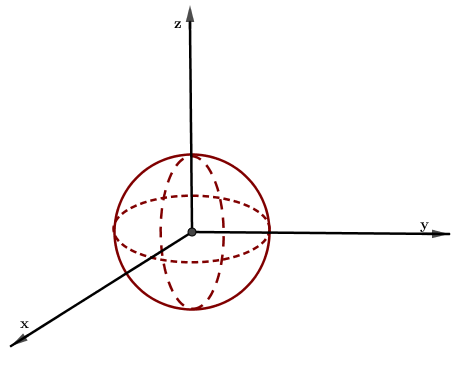
\includegraphics[width=8cm]{d7.png}, 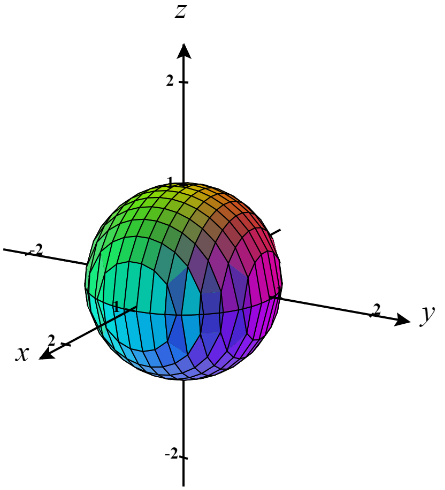
\includegraphics[width=6 cm]{f9.png}}
\end{center}
Zapreminu sfere računamo po formuli:
$$V = 2\iint \limits_D \sqrt{r^{2} - x^2 - y^2 },$$
gdje je oblast integracije $D$: $x^2 + y^2 = r^2.$\\
Uvedimo polarne koordinate:
$$x = \rho \cos{\varphi}$$
$$y = \rho \sin{\varphi}$$
 $$\mathrm dxdy = \rho  \mathrm d \rho  \mathrm d\varphi$$
 
 Iz $x^2 + y^2 = r^2$ dobijamo:
 $$0\leq \rho\leq r \hspace{1 cm} 0\leq \varphi\leq 2\pi.$$
 $$V = 2\iint \limits_D \sqrt{r^{2} - x^2 - y^2 } = 2\iint \limits_D \sqrt{r^{2} - (x^2 + y^2) }$$
  $$ = 2 \int\limits_{0}^{2\pi } d\varphi \int\limits_{0}^{r}\sqrt{r^{2}  - \rho^{2}} d\rho =\left|
\begin{array}{ccc}
Smjena: \\
 r^2 - \rho^{2} = t^{2}  \Rightarrow \rho\mathrm{d\rho}= -t \mathrm{dt} \\
  \end{array}\right |\\$$
  $$ = -2\int\limits_{0}^{2\pi } d\varphi \int\limits_{(0)}^{(r)} t^{2}   dt = -2\int\limits_{0}^{2\pi } d\varphi  \frac{\sqrt{r^{2}  - \rho^{2}}^{3}}{3}\underset{0}{\overset{r}{ \bigg\vert}} $$
  $$= -\frac{2}{3}\int\limits_{0}^{2\pi } d\varphi ( 0 -r^{3}) = \frac{2r^{3}}{3}\cdot 2\pi = \frac{4r^{3}\pi}{3}. $$
 
\hskip 12 cm $\blacktriangleleft$ \\

\begin{tcolorbox}[colback=brown!35!white,colframe=white!75!white,title= $$\bullet \bullet \bullet$$]
         \begin{zadatak}
Izračunati zapreminu tijela ograničenog sa:\\
$z = 1-x^2 - y^2, $ $y=x$, $y= \sqrt{3}x$ i $z=0.$
\end{zadatak}
\end{tcolorbox}
\emph{Rješenje: }
\begin{center}
\tcbox[ colframe=red, colback=white!50!white!30]{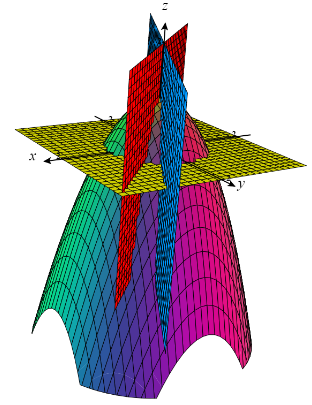
\includegraphics[width=5cm]{d12.png},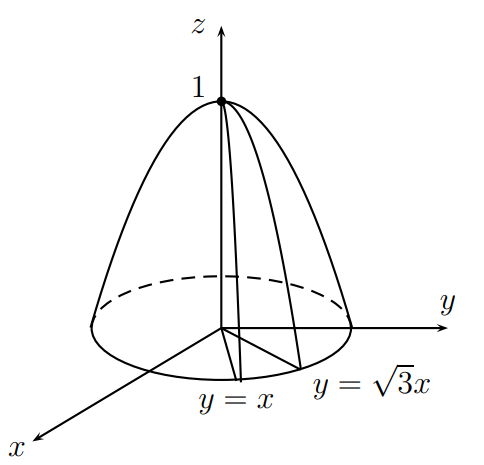
\includegraphics[width=6cm]{d11.png}}
\end{center}
Zapreminu računamo po formuli:
$$V = \iint_{D} (1-x^2 - y^2)\mathrm{dx}\mathrm{dy},$$
gdje  oblast $D$ dobijamo kao presjek površi $z = 1-x^2 - y^2, $ i $z=0$, odnosno:
$$D: x^2 + y^2 =1, \hspace{0.5 cm} y=x, \hspace{0.5 cm} y= \sqrt{3}x$$ 
Oblast $D  $ predstavljena sljedećom slikom:
\begin{center}
\tcbox[ colframe=red, colback=white!50!white!30]{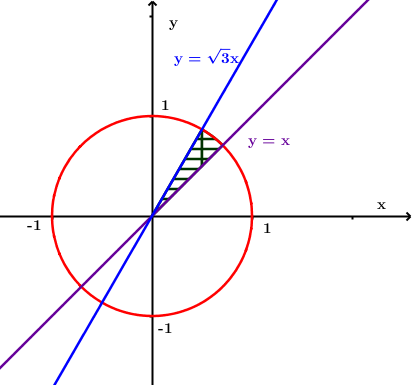
\includegraphics[width=7cm]{d13.png}}
\end{center}
Uvedimo polarne koordinate:
$$x = r \cos{\varphi}$$
$$y = r \sin{\varphi}$$
 $$\mathrm dxdy = r  \mathrm d r  \mathrm d\varphi$$
Dakle, iz $xy$ ravni, tj. oblasti $D$ sada možemo odrediti granice za $r$  i $\varphi$:

Iz $x^2 + y^2 =1 $ dobijamo da je:
 $$0\leq r \leq 1$$
 Iz $$y=x \Rightarrow \varphi = \frac{\pi}{4}$$
 $$y=\sqrt{3}x \Rightarrow \varphi = \frac{\pi}{3}$$
  $$\frac{\pi}{4}\leq \varphi \leq \frac{\pi}{3}$$

 Stoga je tražena zapremina:
$$ V  	=\iint\limits_{ D }\left( 1-x^{2}-y^{2}\right) dx dy = 	\iint\limits_{ D }\left( 1-(x^{2}+y^{2})\right) dx dy$$ 	   
  	$$ =\int\limits_{\frac{\pi}{4}}^{\frac{\pi}{3} } d\varphi \int\limits_{0}^{1}( 1-r^{2})r dr =\int\limits_{\frac{\pi}{4}}^{\frac{\pi}{3} }\left(\frac{r^{2}  }{2} - \frac{r^{4}  }{4} \right) \underset{0}{\overset{1 }{ \bigg\vert}}d\varphi $$
  	$$ =\int\limits_{\frac{\pi}{4}}^{\frac{\pi}{3} }d\varphi \left(\frac{1}{2} - \frac{1}{4}\right) = \frac{1}{4} \left(\frac{\pi}{3} - \frac{\pi}{4}\right) = \frac{\pi}{48}  .$$ 

\hskip 12 cm $\blacktriangleleft$ \\
\newpage
\begin{center}
\tcbox[ colframe=red, colback=white!50!white!30]{\LARGE{PRIMJENA TROJNOG INTEGRALA}}
\end{center}
\begin{tcolorbox}[enhanced,attach boxed title to top center={yshift=-3mm,yshifttext=-1mm},
  colback=yellow!15!white,colframe=red!755!yellow,colbacktitle=brown!90!white,
  title=Zapremina,fonttitle=\bfseries,
  boxed title style={size=small,colframe=red!50!black} ]
   Zapreminu tijela ograničenog sa površi $\Omega$ računamo   po formuli:

$$ V=\iiint\limits_\Omega dx dy dz.$$ 
\end{tcolorbox}
\begin{tcolorbox}[colback=brown!35!white,colframe=white!75!white,title= $$\bullet \bullet \bullet$$]
         \begin{zadatak}
Izračunati zapreminu tijela ograničenog sa:\\
$  x^2 + y^2 + z^2 = 1,$ $z =\sqrt{ x^2 + y^2} .$
\end{zadatak}
\end{tcolorbox}
\emph{Rješenje: }
\begin{center}
\tcbox[ colframe=red, colback=white!50!white!30]{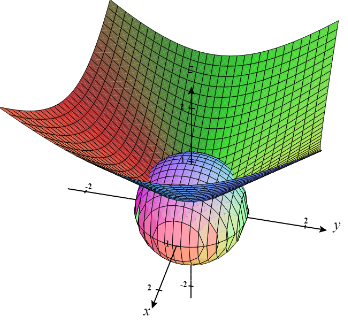
\includegraphics[width=6cm]{f1.png},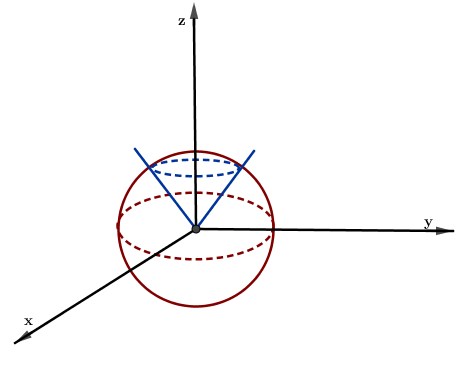
\includegraphics[width=6cm]{f2.png}}
\end{center}
Uvedimo sferne koordinate:
$$x = r\cos{\varphi} \sin{\theta}$$
$$y = r\sin{\varphi} \sin{\theta}$$
$$z = r \cos{\theta}$$
$$|J| = r^{2}\sin{\theta}$$
Iz $x^2 + y^2 + z^2 = 1 \Rightarrow r^2 = 1\Rightarrow r = 1. $
Stoga su granice za $r$:
$$0\leq r\leq 1.$$
Kako nemamo ograničenja za ugao $\varphi,$ to uzimamo maksimalne granice, tj.
$$0\leq \varphi\leq 2\pi.$$
Granice za ugao $\theta$ (otklon od $z$ ose) određujemo u ravni $yOz$. To dobijamo iz jednačine presjeka sfere
$x^{2} + y^{2} + z^{2} = 1 $ i konusa $ z = \sqrt{x^{2} + y^{2}} . $
Odnosno, imamo:
$$z = \sqrt{x^{2} + y^{2}} \Rightarrow z^2 = x^{2} + y^{2}$$
Dobijeni izraz iz jednačine konusa sada uvrstimo u jednačinu sfere: 
$$x^{2} + y^{2} + z^{2} = 1 \Rightarrow 2z^2 = 1 \Rightarrow z^2 = \frac{1}{2} \Rightarrow z =   \frac{\sqrt{2}}{2} $$

Treba nam sada još vrijednost za $y$ u toj tački i to ćemo dobiti kad u jednu od jednačina   uvrstimo $z = \frac{\sqrt{2}}{2}$ i $x = 0 $ :
$$x^{2} + y^{2} + z^{2} = 1 $$
Za  $z = \frac{\sqrt{2} }{2}$ i $x = 0 $ vrijedi:
$$0 + y^{2} + \frac{\sqrt{2}}{2}^{2} = 1 $$
$$\Rightarrow  y^{2} = 1 - \frac{1}{2}   $$
$$\Rightarrow  y^{2} =  \frac{1}{2} \Rightarrow y= \frac{\sqrt{2}}{2} . $$
Pa ugao $\theta$ ćemo izračunati  na osnovu dobijenih vrijednosti za $z$ i $y$ u toj presječnoj tački, odnosno:
$$\tg{\omega} = \frac{z}{y} = \frac{\frac{\sqrt{2}}{2}}{\frac{\sqrt{2}}{2}} = 1 \Rightarrow \omega = \frac{\pi}{4}$$
A kako vrijedi da je $\omega + \theta = \frac{\pi}{2},$ to implicira da je $\theta = \frac{\pi}{4},$ što je krajnja (gornja granica ) za ugao $\theta$, a početna (donja) granica je očigledno $0.$
Dakle, vrijedi:
$$0\leq \theta \leq \frac{\pi}{4}.$$
Pa je tražena zapremina:
$$V=\iiint \limits_{\Omega}    \mathrm dx \mathrm dy \mathrm dz = \iiint \limits_{ \Omega' } r^{2}\sin{\theta}\mathrm dr\mathrm d\varphi \mathrm d\theta    $$
$$= \int\limits_{0}^{2\pi} \mathrm d\varphi \int\limits_{0}^{1} r^{2}\mathrm dr \int\limits_{0}^{\frac{\pi}{4}}  \sin{\theta} \mathrm d\theta=    \int\limits_{0}^{2\pi} \mathrm d\varphi \int\limits_{0}^{1} r^{2}\mathrm dr (-\cos{\theta})\underset{0}{\overset{ \frac{\pi}{4} }{ \bigg\vert}}  $$

$$  \int\limits_{0}^{2\pi} \mathrm d\varphi \int\limits_{0}^{1} r^{2}\mathrm dr \left(-\frac{\sqrt{2}}{2} + 1\right)  =   \int\limits_{0}^{2\pi} \mathrm d\varphi \frac{r^3}{3} \left(-\frac{\sqrt{2}}{2} + 1\right)\underset{0}{\overset{ 1 }{ \bigg\vert}} = \frac{1}{3} \cdot 2\pi \cdot \left(-\frac{\sqrt{2}}{2} + 1\right) = \frac{(2 -\sqrt{2})\pi  }{3} .$$
\hskip 12 cm $\blacktriangleleft$ \\




 

\begin{tcolorbox}[colback=brown!35!white,colframe=white!75!white,title= $$\bullet \bullet \bullet$$]
         \begin{zadatak}
Izračunati zapreminu tijela ograničenog sa:\\
$  z= 6 - x^2 - y^2  ,$ $z^{2} =  x^2 + y^2   $ za $z\geq 0.$
\end{zadatak}
\end{tcolorbox}
\emph{Rješenje: }
\begin{center}
\tcbox[ colframe=red, colback=white!50!white!30]{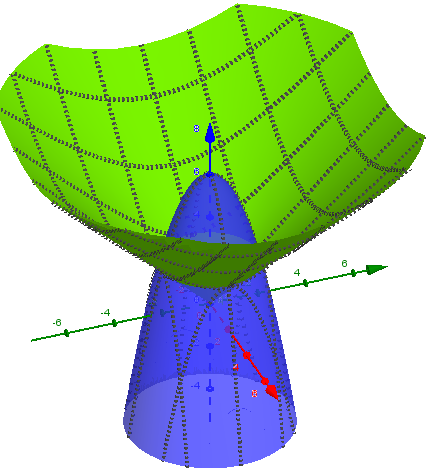
\includegraphics[width=5cm]{f3.png},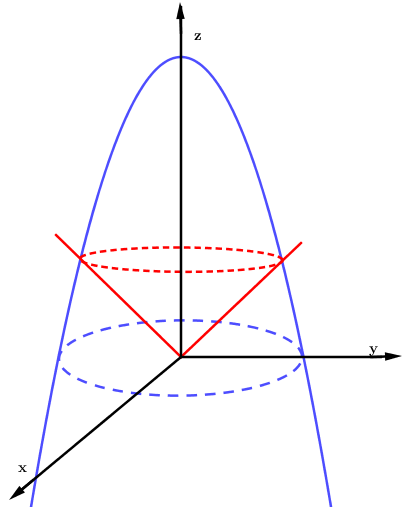
\includegraphics[width=5cm]{f5.png}}
\end{center}
Uvedimo cilindrične koordinate:
$$x= r\cos{\varphi}$$
$$y= r\sin{\varphi}$$
$$z=z$$
$$|J|= r$$
Da bismo odredili granice za $r$ i $\varphi$, moramo odrediti jednačinu presjeka površi(paraboloida i konusa), odnosno trebamo riješiti sistem:
$$z= 6 - x^2 - y^2 \hspace{0.3 cm} i \hspace{0.3 cm} z^2  =  x^2 + y^2   $$
Iz $z= 6 - x^2 - y^2$ vrijedi:
$$z-6 = -(x^2 + y^2) \Rightarrow x^2 + y^2 = 6-z $$
Sada, ovako dobijen izraz uvrštavamo u $ z^2  =  x^2 + y^2  $ , pa ćemo dobiti:
$$z^2  = 6-z \Longleftrightarrow z^2 +z - 6 =0 \Rightarrow z_{1,2}  = \frac{-1\pm \sqrt{25}}{2} \Rightarrow z_1 = 2 \hspace{0.3 cm} z_2 = -3. $$
Dakle, jednačina presjeka je: $$x^2 + y^2 = 2^2  \Longleftrightarrow r^2 = 2^2 \Longleftrightarrow r=2. $$
Pa su granice za $r:$
$$0\leq r \leq 2.$$
Kako nema ograničenja za ugao, to je:
$$0\leq \varphi \leq 2\pi.$$
Konačno, granice za $z$ su:
$$z \underset{konus}{\overset{ paraboloid }{ \bigg\vert}} \Rightarrow z \underset{\sqrt{x^2 + y^2}}{\overset{ 6 - (x^2 + y^2 )}{ \bigg\vert}} \Rightarrow z \underset{r }{\overset{ 6 - r^2  }{ \bigg\vert}}.$$
Tražena zapremina je:
$$V =\iiint \limits_{\Omega}    \mathrm dx \mathrm dy \mathrm dz = \iiint \limits_{\Omega'}    r \mathrm dr \mathrm d\varphi \mathrm dz $$
$$= \int\limits_{0}^{2\pi} \mathrm d\varphi \int\limits_{0}^{2} r\mathrm dr \int\limits_{  r  }^{   6 - r^2 }   \mathrm dz=  \int\limits_{0}^{2\pi} \mathrm d\varphi \int\limits_{0}^{2 } r\mathrm dr(6-r^2 - r )  $$

$$=\int\limits_{0}^{2\pi} \mathrm d\varphi \int\limits_{0}^{2 } (6r - r^3 - r^2  )\mathrm dr     =  \int\limits_{0}^{2\pi} \mathrm d\varphi \left( 6\frac{ r^2  }{2} -  \frac{ r^4  }{4} - \frac{ r^3  }{3} \right)\underset{0}{\overset{ 2}{ \bigg\vert}}   $$
$$= \int\limits_{0}^{2\pi} \mathrm d\varphi\left(12 - 4 - \frac{ 8}{3}  \right) = 2\pi \cdot \frac{16 }{3} = \frac{32\pi}{3} .$$
\hskip 12 cm $\blacktriangleleft$ \\




\begin{tcolorbox}[colback=brown!35!white,colframe=white!75!white,title= $$\bullet \bullet \bullet$$]
         \begin{zadatak}
Izračunati zapreminu tijela ograničenog sa:\\
$  z= 1 - x^2 - y^2  ,$ $z  =  x^2 + y^2  .$
\end{zadatak}
\end{tcolorbox}
\emph{Rješenje: }
\begin{center}
\tcbox[ colframe=red, colback=white!50!white!30]{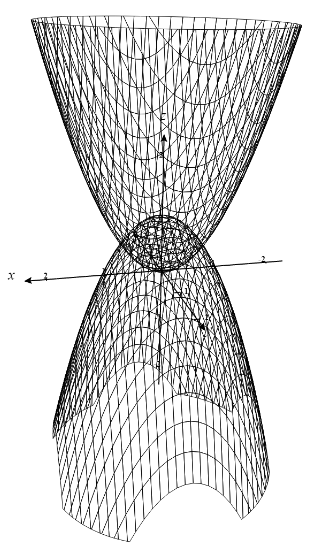
\includegraphics[width=4cm]{f7.png},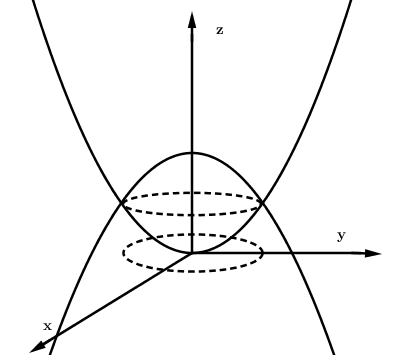
\includegraphics[width=6cm]{f8.png}}
\end{center}
Uvedimo cilindrične koordinate:
$$x= r\cos{\varphi}$$
$$y= r\sin{\varphi}$$
$$z=z$$
$$|J|= r$$
Da bismo odredili granice za $r$ i $\varphi$, moramo odrediti jednačinu presjeka površi, odnosno trebamo riješiti sistem:
$$z= 1 - x^2 - y^2 \hspace{0.3 cm} i \hspace{0.3 cm} z  =  x^2 + y^2   $$
Imamo, dakle, da vrijedi:
$$x^2 + y^2  =  1 - x^2 - y^2 \Rightarrow 2x^2 + 2y^2  = 1 \Rightarrow x^2 + y^2 = \frac{1}{2} \Rightarrow x^2 + y^2 =   \left(\frac{\sqrt{2}}{2}\right)^2$$
$$\Rightarrow r^2 =\left(\frac{\sqrt{2}}{2}\right)^2 \Rightarrow r = \frac{\sqrt{2}}{2}.  $$
Stoga, granice za $r$ su:
$$0\leq r \leq \frac{\sqrt{2}}{2}.$$
Nemamo ograničenja za ugao $\varphi$, pa je:
$$0\leq \varphi \leq 2\pi.$$
Dok su granice za $z$ :
$$x^2 + y^2\leq z \leq 1 - x^2 - y^2$$
Odnosno, nakon uvođenja cilindričnih koordinata:
$$r^2\leq z \leq 1 -r^2.$$
Stoga, tražena zapremina je:
$$V =\iiint \limits_{\Omega}    \mathrm dx \mathrm dy \mathrm dz = \iiint \limits_{\Omega'}    r \mathrm dr \mathrm d\varphi \mathrm dz $$
$$= \int\limits_{0}^{2\pi} \mathrm d\varphi \int\limits_{0}^{\frac{\sqrt{2}}{2}} r\mathrm dr \int\limits_{  r^2 }^{   1 - r^2 }   \mathrm dz=  \int\limits_{0}^{2\pi} \mathrm d\varphi \int\limits_{0}^{\frac{\sqrt{2}}{2} } r\mathrm dr(1-r^2 - r^2)  $$

$$=\int\limits_{0}^{2\pi} \mathrm d\varphi \int\limits_{0}^{\frac{\sqrt{2}}{2} } (r -2r^3  )\mathrm dr     =  \int\limits_{0}^{2\pi} \mathrm d\varphi \left( \frac{ r^2  }{2} - 2\frac{ r^4  }{4}\right)\underset{0}{\overset{ \frac{\sqrt{2}}{2} }{ \bigg\vert}}   $$
$$= \int\limits_{0}^{2\pi} \mathrm d\varphi\left(\frac{ 1  }{4} - \frac{ 1  }{8}\right) = 2\pi \cdot \frac{ 1  }{8} = \frac{\pi}{4} .$$
\hskip 12 cm $\blacktriangleleft$ \\


















\begin{tcolorbox}[colback=brown!35!white,colframe=white!75!white,title= $$\bullet \bullet \bullet$$]
         \begin{zadatak}
Izračunati zapreminu tijela ograničenog sa:\\
$   x^2 + y^2 + z^2 \leq 1  ,$ $  x^2 + y^2 + z^2 \leq 2z .$
\end{zadatak}
\end{tcolorbox}
\emph{Rješenje: }
Uvedimo cilindrične koordinate:
$$x= r\cos{\varphi}$$
$$y= r\sin{\varphi}$$
$$z=z$$
$$|J|= r$$
\begin{center}
\tcbox[ colframe=red, colback=white!50!white!30]{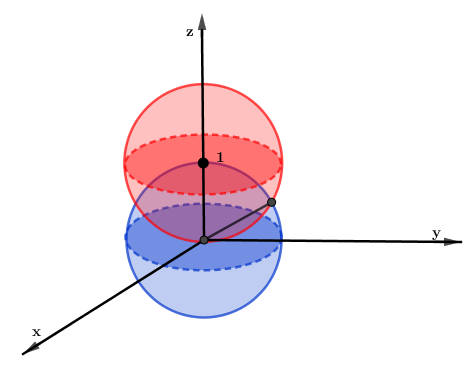
\includegraphics[width=8cm]{e13.png} }
\end{center}
Dakle, imamo da vrijedi:
$$ x^2 + y^2 + z^2 \leq 2z \Longleftrightarrow x^2 + y^2 + (z-1)^2 \leq 1$$
Sada nađimo granice za $z$. Primijetimo da je početna granica za $z$ zapravo donja polovina crvene sfere,odnosno, kako smo uveli cilindrične koordinate, to će biti :
$$r^2 + (z-1)^2 = 1$$
$$ (z-1)^2 = 1 - r^2  $$
$$z -1 = \pm \sqrt{1 - r^2}$$
Ali, kao što je rečeno, početna granica za $z$ je donja polovina crvene sfere, pa uzimamo negativnu vrijednost:
$$z -1 = - \sqrt{1 - r^2}$$
$$z   = 1 - \sqrt{1 - r^2}$$
Dakle, unutar tražene oblasti integracije, našli smo da je početna granica za $z$:  
$$z   = 1 - \sqrt{1 - r^2}$$
Kad je riječ o krajnjoj (gornjoj ) granici za $z$, vidimo da je ona određena gornjom polovinom plave (centralne sfere), pa vrijedi:
$$x^2 + y^2 + z^2 = 1$$
$$r^2 + z^2 = 1$$
$$  z^2 = 1 - r^2$$
$$  z  =\pm \sqrt{ 1 - r^2}$$
 Ali, kao što je rečeno, gornja granica za $z$ je gornja polovina plave sfere, pa uzimamo pozitivnu vrijednost:
$$  z  =  \sqrt{ 1 - r^2}$$
Prema tome, granice za $z$ su:
$$1 - \sqrt{1 - r^2} \leq z \leq \sqrt{ 1 - r^2}. $$
Sada nađimo granice za r. Donja granica je, naravno, minimalna, odnosno 0. Gornja granica za r je određena jdnačinom presjeka donjeg dijela crvene i gornjeg dijela plave sfere, tj:
$$1 - \sqrt{1 - r^2} = \sqrt{ 1 - r^2}$$
$$2 \sqrt{ 1 - r^2} = 1 \hspace{0.5 cm}/^2$$
$$4(1-r^2) =1$$
$$1-r^2 = \frac{1}{4} \Rightarrow r = \frac{\sqrt{3}}{2}.$$
Stoga, granice za $r$ su:
$$0\leq r \leq \frac{\sqrt{3}}{2}.$$
Kako nemamo ograničenja za ugao $\varphi,$ to uzimamo maksimalne granice:

$$ 0\leq \varphi \leq 2\pi.$$
Pa je tražena zapremina:
$$V =\iiint \limits_{\Omega}    \mathrm dx \mathrm dy \mathrm dz = \iiint \limits_{\Omega'}    r \mathrm dr \mathrm d\varphi \mathrm dz $$
$$= \int\limits_{0}^{2\pi} \mathrm d\varphi \int\limits_{0}^{\frac{\sqrt{3}}{2}} r\mathrm dr \int\limits_{1 - \sqrt{1 - r^2}}^{  \sqrt{1 - r^2}}   \mathrm dz= 2\pi \int\limits_{0}^{\frac{\sqrt{3}}{2} } r\mathrm dr(2\sqrt{1 - r^2} -1)  $$

$$= 2\pi \left(\int\limits_{0}^{\frac{\sqrt{3}}{2} } 2r  \sqrt{1 - r^2} \mathrm{dr} - \int\limits_{0}^{\frac{\sqrt{3}}{2} }r\mathrm{dr} \right) = 2\pi \left(-\frac{2\sqrt{1-r^2}^{3}}{3}\underset{0}{\overset{ \frac{\sqrt{3}}{2} }{ \bigg\vert}}  - \frac{r^2}{2} \underset{0}{\overset{ \frac{\sqrt{3}}{2} }{ \bigg\vert}}\right) $$
$$= 2\pi \left(\frac{7}{12} - \frac{3}{8}\right) = \frac{5\pi}{12}.$$
\hskip 12 cm $\blacktriangleleft$ \\



\end{document}